\section{Koordinationsverbindungen II - Ligandenfeldtheorie}
\authors{Lynn Meeder, Patricia Mühren}

Die Kristallfeldtheorie beschreibt Koordinationsverbindungen, wobei die Liganden klassisch betrachtet werden und das Zentralatom/-ion quantenmechanisch beschrieben wird. Ein genaueres Modell ist die Ligandenfeldtheorie, in der sowohl das Zentralatom/-ion als auch die Liganden sowie ihre Wechselwirkungen quantenmechanisch betrachtet werden.

\subsection{Ligandenfeldtheorie und 18-Elektronen-Regel}

Analog zur Oktettregel lässt sich die 18-Elektronen-Regel für Nebengruppenelemente formulieren. Wenn das System 18 Valenzelektronen hat, so ist die Komplexbildung stabil \cite{Huheey}.

Die Liganden sorgen auch in diesem Modell, genau wie bei der Kristallfeldtheorie, für eine Aufspaltung der Energieniveaus der $d$-Orbitale des Zentralatoms/-ions. Dabei bilden die $d_{z^2}$- und $d_{x^2-y^2}$-Orbitale des Zentralatoms/-ions mit zwei symmetrieadaptierten Linearkombinationen (SALCs) der Liganden zwei bindende und zwei antibindende Orbitale. Die bindenden Orbitale liegen auf einem energetisch niedrigeren Niveau und werden als $e_g$-Orbitale bezeichnet. Auf einem höheren Energieniveau liegen die antibindenden $e^*_g$-Orbitale. Die energetisch niedriger liegenden $d_{xy}$-, $d_{xz}$- und $d_{yz}$-Orbitale  werden als $t_{2g}$-Orbitale bezeichnet und sind nicht bindend.

Das unbesetzte $s$-Orbital des Zentralatoms/-ions bildet mit einem der SALCs der Liganden das komplett symmetrische $a_{1g}$-Orbital und das entsprechende antibindende $a^*_{1g}$-Orbital. Die drei unbesetzten $p$-Orbitale des Zentralatoms/-ions bilden mit drei SALCs der Liganden die bindenden, dreifach entarteten $t_{1u}$-Orbitale und ebenfalls die entsprechenden antibindenden $t^*_{1u}$-Orbitale.

Die Aufspaltungsenergie $\Delta_0$ beschreibt die Energiedifferenz zwischen den $e^*_g$- und $t_{2g}$-Orbitalen (siehe Abbildung \ref{Level}).

\begin{dsafigure}
	\centering
	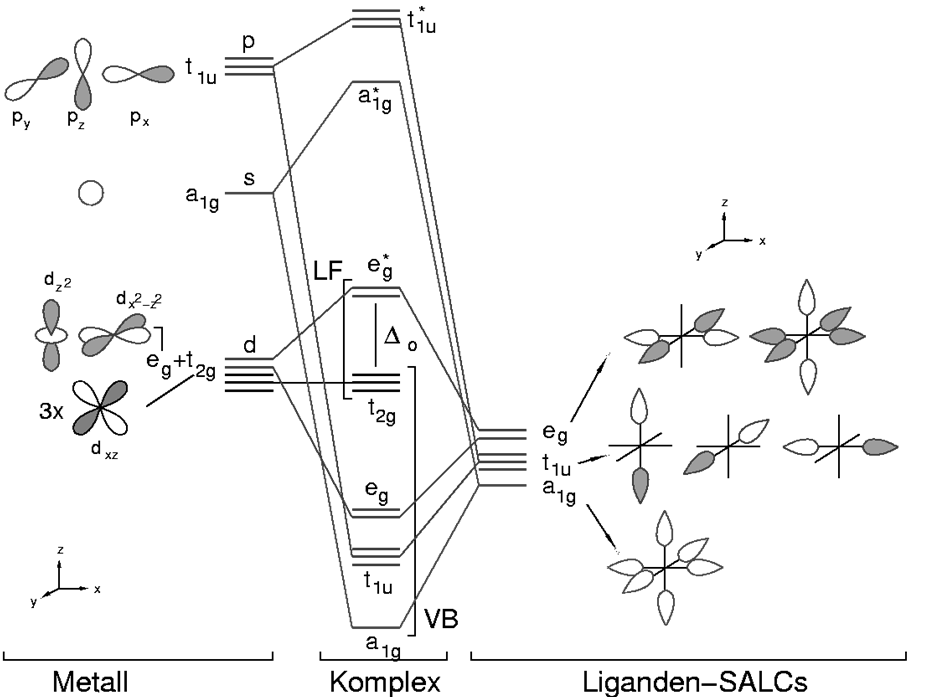
\includegraphics[width=\columnwidth]{EnergielevelKomplex.png}
	\caption{Die Molekülorbitale einer oktaedrischen Koordinationsverbindung \cite{Chemie_der_Metalle}}
	\label{Level}
\end{dsafigure}

Wie in Abbildung \ref{Level} sichtbar, gibt es sechs bindende und drei nicht bindende Orbitale. Die stärkste Bindung erhält man also, wenn diese neun Orbitale voll -- also mit 18 Elektronen -- besetzt sind. Damit lässt sich nun die 18-Elektronen-Regel begründen. 

Diese Regel gilt nun allerdings wie Abbildung \ref{Level}  nur für oktaedrische Komplexverbindungen. Bei anderen Koordinationsgeometrien unterscheidet sich das Molekülorbitalschema und dadurch kann eine andere Zahl an Valenzelektronen stabil sein.


